\documentclass[tikz,border=8pt]{standalone}
% Shared look for every TikZ diagram. Load with \input{../../tools/tikz-style.tex}
\usepackage[T1]{fontenc}
\usepackage{lmodern}
\renewcommand{\sfdefault}{lmr}  % diagrams use the same serif as the text
\usetikzlibrary{arrows.meta, positioning, shapes.geometric, calc, fit, backgrounds}
\definecolor{cblue}{HTML}{4C78A8}
\definecolor{corange}{HTML}{F58518}
\definecolor{cgreen}{HTML}{54A24B}
\definecolor{cred}{HTML}{E45756}
\definecolor{cpurple}{HTML}{B279A2}
\definecolor{cgrey}{HTML}{6B6B6B}
\tikzset{
  every picture/.style={font=\sffamily, line width=1.2pt},
  box/.style={draw=#1, fill=#1!12, rounded corners=4pt, align=center, inner sep=7pt, minimum height=1.1cm},
  box/.default=cgrey,
  arrow/.style={-{Stealth[length=3mm]}, draw=cgrey, line width=1.4pt},
  title/.style={font=\sffamily\bfseries\Large},
  note/.style={font=\sffamily\small, text=cgrey, align=center},
}
\AtBeginDocument{\hyphenpenalty=10000 \exhyphenpenalty=10000}

\begin{document}
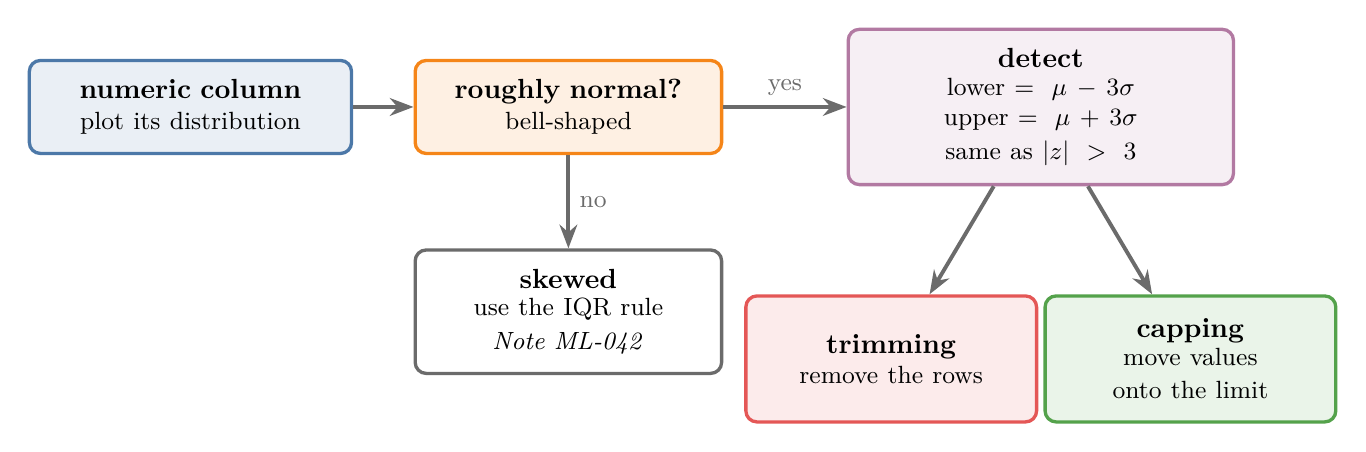
\begin{tikzpicture}
  \node[box=cblue, text width=3.6cm] (col) at (0,0) {\textbf{numeric column}\\[-1pt]\small plot its distribution};
  \node[box=corange, text width=3.4cm] (q) at (4.8,0) {\textbf{roughly normal?}\\[-1pt]\small bell-shaped};
  \draw[arrow] (col) -- (q);
  \node[box=cgrey, fill=white, text width=3.4cm] (iqr) at (4.8,-2.6) {\textbf{skewed}\\[-1pt]\small use the IQR rule\\ \textit{Note ML-042}};
  \draw[arrow] (q) -- node[right, note] {no} (iqr);
  \node[box=cpurple, text width=4.4cm] (lim) at (10.8,0) {\textbf{detect}\\[-1pt]\small lower $= \mu - 3\sigma$\\ upper $= \mu + 3\sigma$\\ same as $|z| > 3$};
  \draw[arrow] (q) -- node[above, note] {yes} (lim);
  \node[box=cred, text width=3.2cm, minimum height=1.6cm] (trim) at (8.9,-3.2) {\textbf{trimming}\\[-1pt]\small remove the rows};
  \node[box=cgreen, text width=3.2cm, minimum height=1.6cm] (cap) at (12.7,-3.2) {\textbf{capping}\\[-1pt]\small move values\\ onto the limit};
  \draw[arrow] (lim) -- (trim); \draw[arrow] (lim) -- (cap);
\end{tikzpicture}
\end{document}
